%========================================================================================
% TU Dortmund, Informatik Lehrstuhl VII
%========================================================================================

\chapter{Das Kapitel 2}
\label{Kapitel 2}
%
Gehetzt sah er sich um. Plötzlich erblickte er den schmalen
Durchgang. Blitzartig drehte er sich nach rechts und verschwand
zwischen den beiden Gebäuden. Beinahe wäre er dabei über den
umgestürzten Mülleimer gefallen, der mitten im Weg lag. Er
versuchte, sich in der Dunkelheit seinen Weg zu ertasten und
erstarrte: Anscheinend gab es keinen anderen Ausweg aus diesem
kleinen Hof als den Durchgang, durch den er gekommen war.


\section{Kapitel 2 - Unterkapitel 1}
\label{Kapitel_2_-_Unterkapitel_1}
%
Er hörte \enquote{leise Schritte} hinter sich. Das bedeutete
nichts Gutes. Wer würde ihm schon folgen, spät in der Nacht und
dazu noch in dieser engen Gasse mitten im übel beleumundeten
Hafenviertel? Gerade jetzt, wo er das Ding seines Lebens gedreht
hatte und mit der Beute verschwinden wollte! Hatte einer seiner
zahllosen Kollegen dieselbe Idee gehabt, ihn beobachtet und
abgewartet, um ihn nun um die Früchte seiner Arbeit zu
erleichtern? Oder gehörten die Schritte hinter ihm zu einem der
unzähligen Gesetzeshüter dieser Stadt, und die stählerne Acht um
seine Handgelenke würde gleich zuschnappen? Er konnte die
Aufforderung stehen zu bleiben schon hören:

\begin{itemize}
  \item Stop
  \item Stop
  \item Stop.
\end{itemize}

Gehetzt sah er sich um. Plötzlich erblickte er den schmalen
Durchgang. Blitzartig drehte er sich nach rechts und verschwand
zwischen den beiden Gebäuden. Beinahe wäre er dabei über den
umgestürzten Mülleimer gefallen, der mitten im Weg lag. Er
versuchte, sich in der Dunkelheit seinen Weg zu ertasten und
erstarrte: Anscheinend gab es keinen anderen Ausweg aus diesem
kleinen Hof als den Durchgang, durch den er gekommen war. Die
Schritte wurden lauter und lauter, er sah eine dunkle Gestalt um
die Ecke biegen. Fieberhaft irrten seine Augen durch die
nächtliche Dunkelheit und suchten einen Ausweg. War jetzt wirklich
alles vorbei, waren alle Mühe und alle Vorbereitungen umsonst \cite{Abramowski:1991}?



    \begin{figure}[t]
    \centering
    \subfigure[]
          {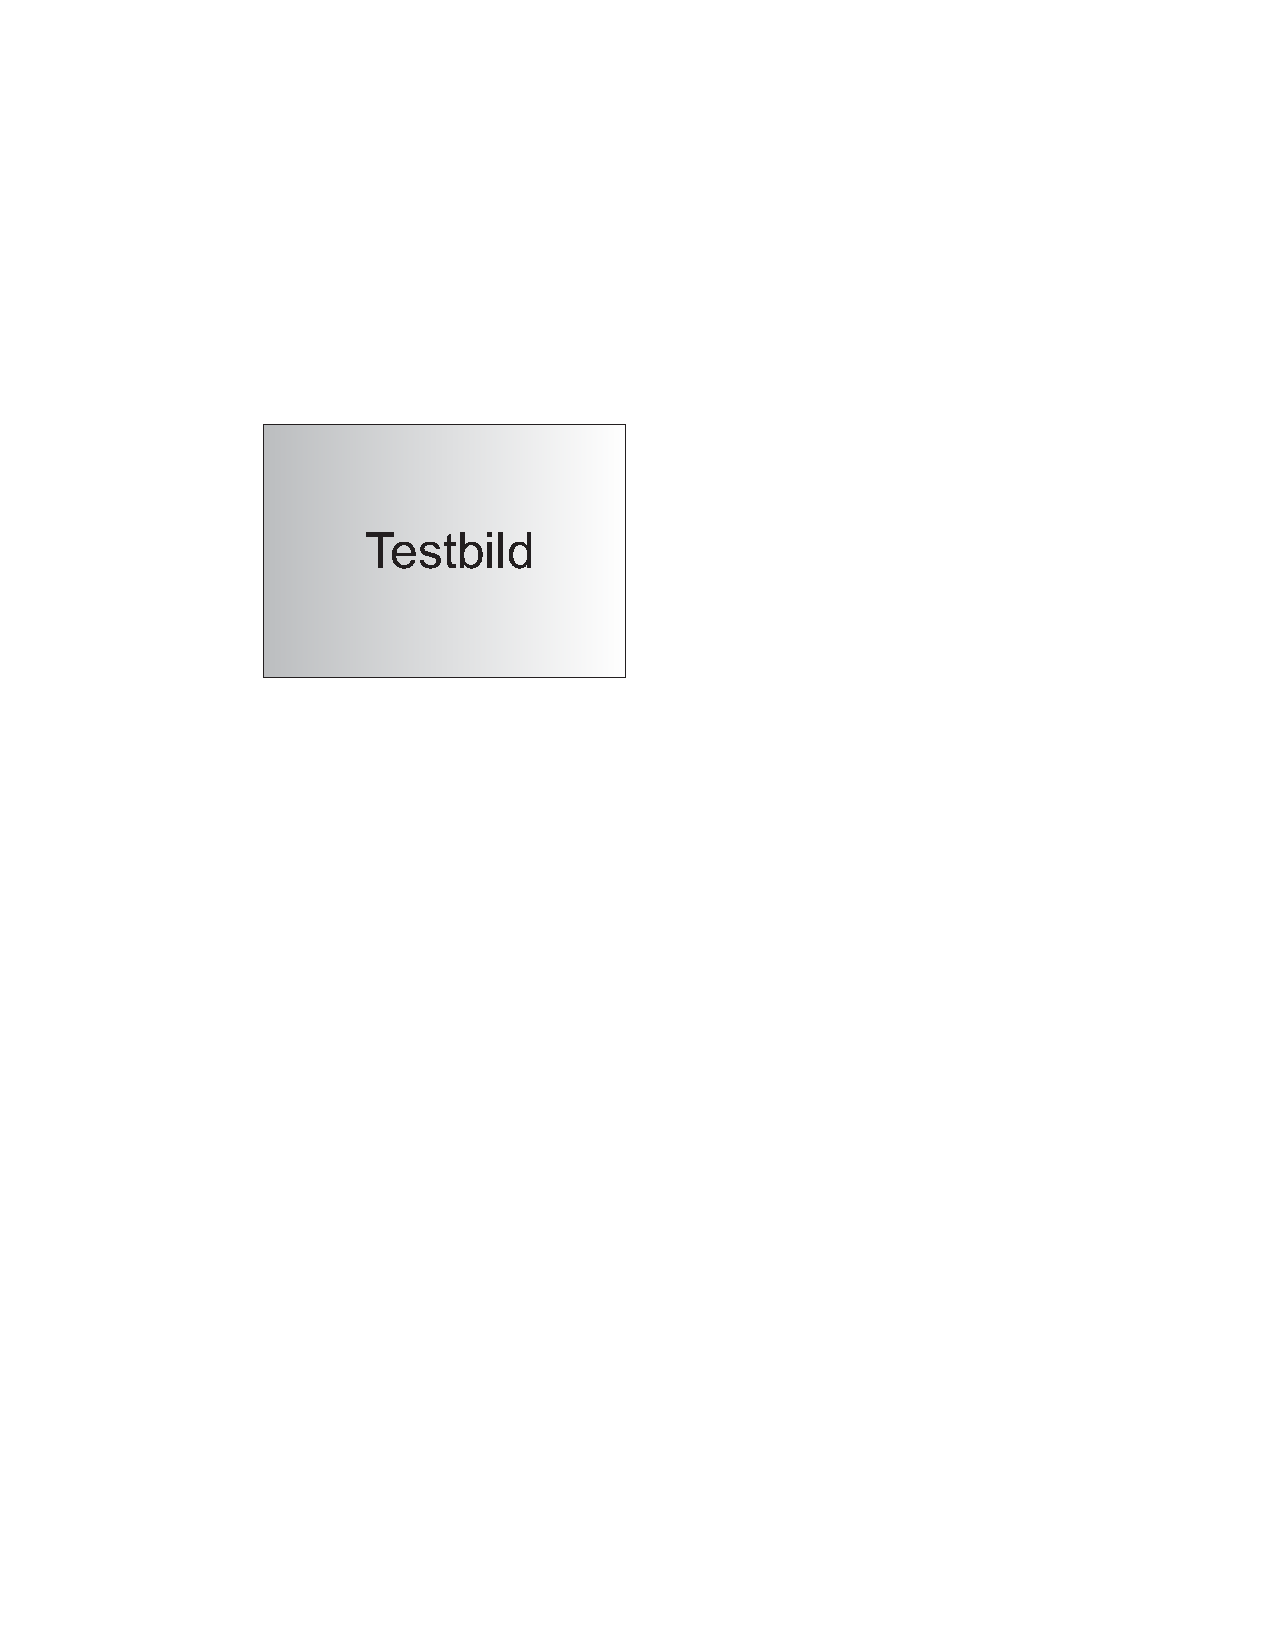
\includegraphics[scale=0.8]{bilder/testbild}\label{fig_testbild_a}
    }
    \hspace{0.5cm}%
    \subfigure[]
         {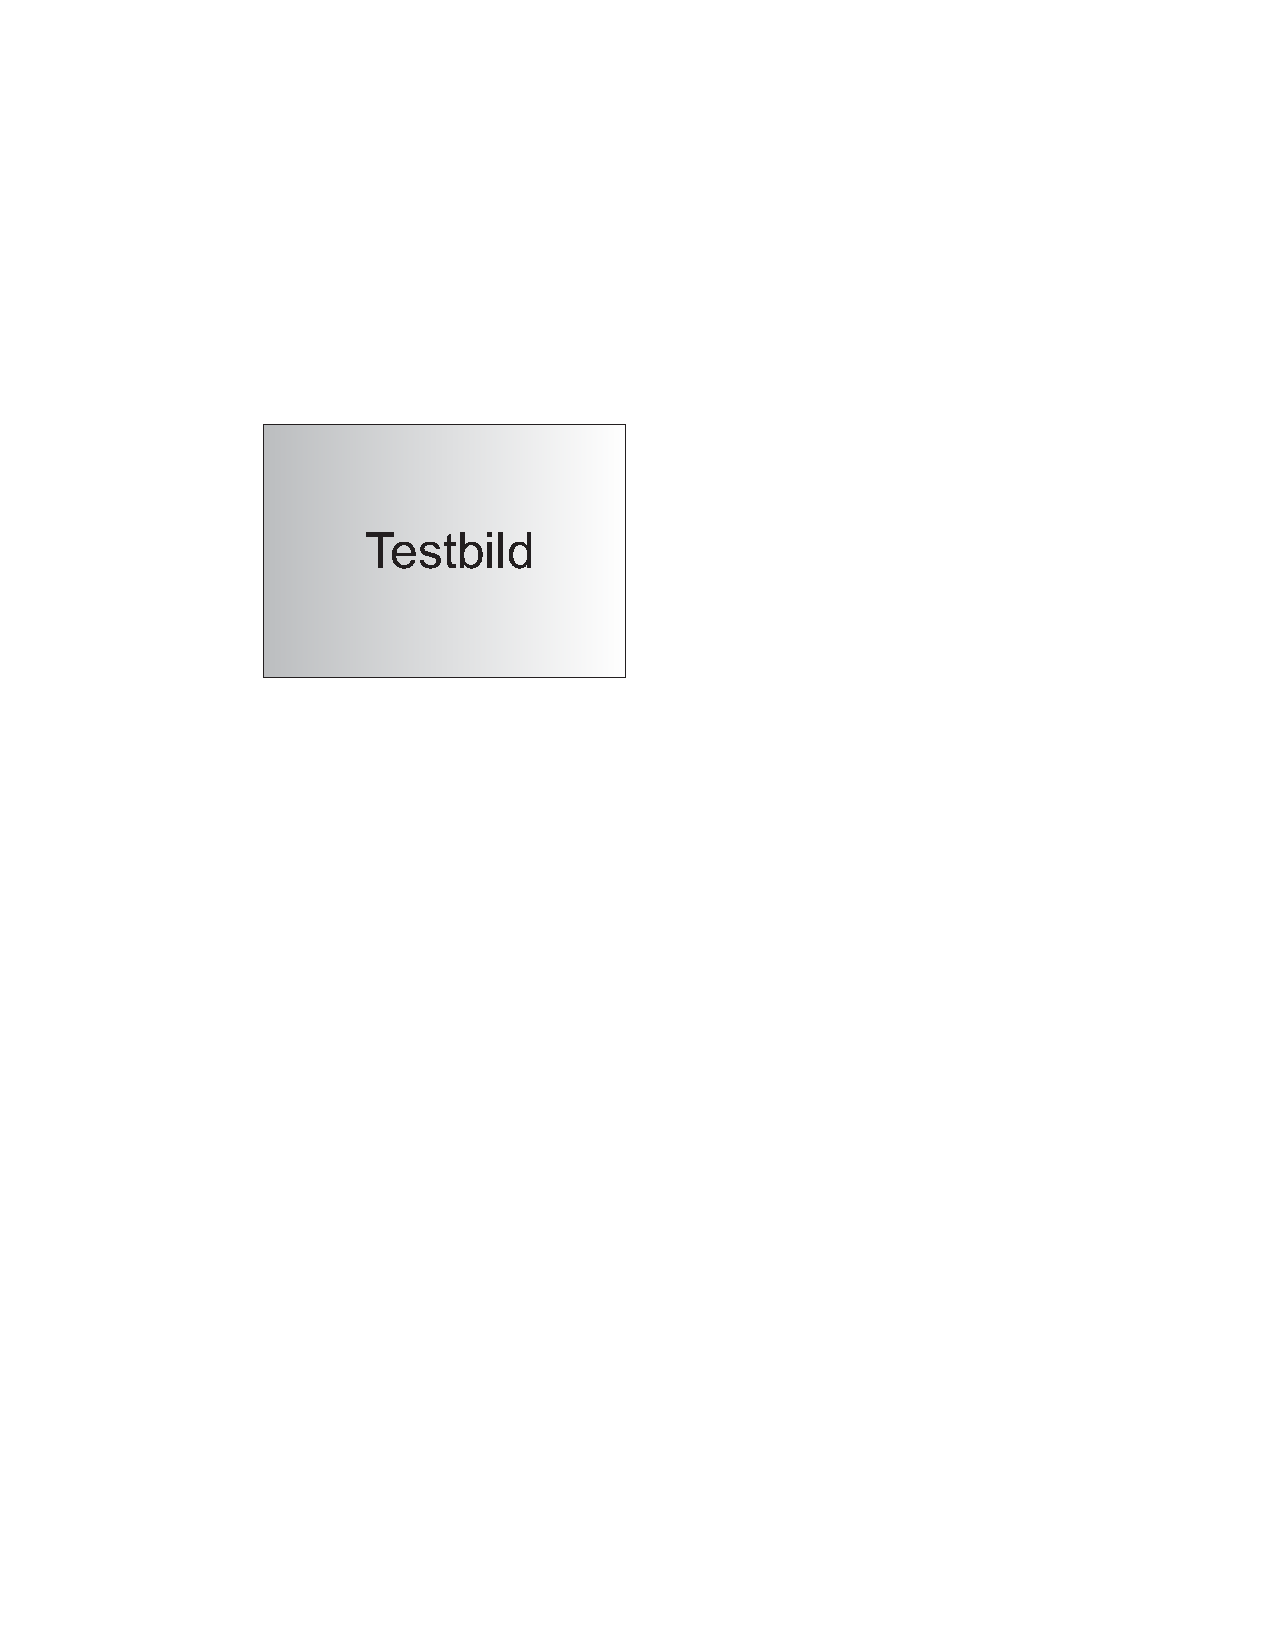
\includegraphics[scale=0.8]{bilder/testbild}\label{fig_testbild_b}
    }
    \caption[Testbilder]{Testbilder}
        \label{fig_testbild}
    \end{figure}

Er presste sich ganz eng an die Wand hinter ihm und hoffte, der
Verfolger würde ihn übersehen, als plötzlich neben ihm mit kaum
wahrnehmbarem Quietschen eine Tür im nächtlichen Wind hin und her
schwang. Könnte dieses der flehentlich herbeigesehnte Ausweg aus
seinem Dilemma sein? Langsam bewegte er sich auf die offene Tür
zu, immer dicht an die Mauer gepresst. Würde diese Tür seine
Rettung werden? Er hörte leise Schritte hinter sich. Das bedeutete
nichts Gutes. Wer würde ihm schon folgen, spät in der Nacht und
dazu noch in dieser engen Gasse mitten im übel beleumundeten
Hafenviertel? Gerade jetzt, wo er das Ding seines Lebens gedreht
hatte und mit der Beute verschwinden wollte! Hatte einer seiner
zahllosen Kollegen dieselbe Idee gehabt, ihn beobachtet und
abgewartet, um ihn nun um die Früchte seiner Arbeit zu
erleichtern? Oder gehörten die Schritte hinter ihm zu einem der
unzähligen Gesetzeshüter dieser Stadt, und die stählerne Acht um
seine Handgelenke würde gleich zuschnappen? Er konnte die
Aufforderung stehen zu bleiben schon hören. Gehetzt sah er sich
um. Plötzlich erblickte er den schmalen Durchgang. Blitzartig
drehte er sich nach rechts und verschwand zwischen den beiden
Gebäuden.


\section{Kapitel 2 - Unterkapitel 2}
\label{Kapitel_2_-_Unterkapitel_2}
%
Er hörte \enquote{leise Schritte} hinter sich. Das bedeutete
nichts Gutes. Wer würde ihm schon folgen, spät in der Nacht und
dazu noch in dieser engen Gasse mitten im übel beleumundeten
Hafenviertel? Gerade jetzt, wo er das Ding seines Lebens gedreht
hatte und mit der Beute verschwinden wollte! Hatte einer seiner
zahllosen Kollegen dieselbe Idee gehabt, ihn beobachtet und
abgewartet, um ihn nun um die Früchte seiner Arbeit zu
erleichtern? Oder gehörten die Schritte hinter ihm zu einem der
unzähligen Gesetzeshüter dieser Stadt, und die stählerne Acht um
seine Handgelenke würde gleich zuschnappen? Er konnte die
Aufforderung stehen zu bleiben schon hören:


    \begin{equation}
        \label{gleichung_nummer_1}
        \mu_{x}(y) = \left\{ \begin{array}{lll}
        4^{\alpha_0} & \qquad \textrm{für} \qquad y \leq 3\\
        \\
        4^{\alpha_1} & \qquad \textrm{für} \qquad y > 3\\
        \end{array} \right.
    \end{equation}
    mit
    \begin{eqnarray}
        \label{gleichung_nummer_2}
        \alpha_0 & = & -\ln 2 \cdot y - \bar{y}\\
        \alpha_1 & = & -\ln 2 \cdot y - \bar{y}\textrm{.}
    \end{eqnarray}



Gehetzt sah er sich um. Plötzlich erblickte er den schmalen
Durchgang. Blitzartig drehte er sich nach rechts und verschwand
zwischen den beiden Gebäuden. Beinahe wäre er dabei über den
umgestürzten Mülleimer gefallen, der mitten im Weg lag. Er
versuchte, sich in der Dunkelheit seinen Weg zu ertasten und
erstarrte: Anscheinend gab es keinen anderen Ausweg aus diesem
kleinen Hof als den Durchgang, durch den er gekommen war. Die
Schritte wurden lauter und lauter, er sah eine dunkle Gestalt um
die Ecke biegen. Fieberhaft irrten seine Augen durch die
nächtliche Dunkelheit und suchten einen Ausweg. War jetzt wirklich
alles vorbei, waren alle Mühe und alle Vorbereitungen umsonst?

Er presste sich ganz eng an die Wand hinter ihm und hoffte, der
Verfolger würde ihn übersehen, als plötzlich neben ihm mit kaum
wahrnehmbarem Quietschen eine Tür im nächtlichen Wind hin und her
schwang. Könnte dieses der flehentlich herbeigesehnte Ausweg aus
seinem Dilemma sein? Langsam bewegte er sich auf die offene Tür
zu, immer dicht an die Mauer gepresst. Würde diese Tür seine
Rettung werden? Er hörte leise Schritte hinter sich. Das bedeutete
nichts Gutes. Wer würde ihm schon folgen, spät in der Nacht und
dazu noch in dieser engen Gasse mitten im übel beleumundeten
Hafenviertel? Gerade jetzt, wo er das Ding seines Lebens gedreht
hatte und mit der Beute verschwinden wollte! Hatte einer seiner
zahllosen Kollegen dieselbe Idee gehabt, ihn beobachtet und
abgewartet, um ihn nun um die Früchte seiner Arbeit zu
erleichtern? Oder gehörten die Schritte hinter ihm zu einem der
unzähligen Gesetzeshüter dieser Stadt, und die stählerne Acht um
seine Handgelenke würde gleich zuschnappen? Er konnte die
Aufforderung stehen zu bleiben schon hören. Gehetzt sah er sich
um. Plötzlich erblickte er den schmalen Durchgang. Blitzartig
drehte er sich nach rechts und verschwand zwischen den beiden
Gebäuden.







%
